\chapter{Frameworks and Tools}\label{Frameworks_and_Tools}
In this chapter, the most important tools and frameworks used within the context of this bachelor thesis will be introduced. First, Eclipse and Eclipse frameworks related to \textsc{Cinco} are listed, followed by a closer look at \textsc{Cinco}. Finally, a tool for creating SCCharts is introduced.
\section{Eclipse and Frameworks} 
Eclipse is an open-source software project released by IBM since 2001, primarily known as an IDE. However, Eclipse also offers a variety of frameworks and plug-ins that can be easily integrated, thanks to Equinox, an implementation of the OSGi R4 specification.~\cite{Guindon.03.09.2023b} Through the easy integration of these already existing or self-created plug-ins and frameworks, developers can create applications without having to implement complex functionalities themselves.

One of this frameworks is the EMF. It is the central technology within Eclipse for MDSD, as it allows for the design of metamodels using the metamodeling language Ecore. The components of these metamodels can be generated as Java-based code and subsequently customized. Additionally, models can be designed and adapted in a tree-like editor. Furthermore, EMF provides a powerful Application Programming Interface (API). As a result, many other projects in the context of MDSD build upon EMF and offer additional functionalities, such as \textsc{Cinco}.~\cite{Guindon.03.09.2023b}~\cite{Brambilla.2017}

Another framework is Xtext which can be used for the development of programming languages and DSLs, by letting programmers define their own languages via a powerful grammar language. It also offers a well-developed infrastructure which includes linker, parser, typechecker, etc., as well as eclipse integration. 

Xtend is an expressive and flexible java dialect. It compiles in java and thus enables any integration of java libraries. It also offers the function of extending existing types without modifying them, hence the name. It also has the same runtime as equivalent Java code and offers other features such as lambda expressions or template expressions.

\section{\textsc{Cinco} SCCE Meta Tooling Framework}
\textsc{Cinco} is a DSL tool to create domain specific graphical modeling tools. It leverages the extensive metamodeling and infrastructure features provided by the EMF, and the Graphiti diagram editor framework, a modeling infrastructure centered around the EMF, in case for representation and editing.~\cite{Wenz.08.09.2023}~\cite{Naujokat.2018}

Every graphical tool created with \textsc{Cinco}, also called \textsc{Cinco} Product, has at its core the Meta Graph Language (MGL) model, from which the Ecore metamodel is ultimately generated. The MGL also defines which components exists in the model and can be created in the editor at the end. The components are all of the type \textit{node}, \textit{container} or \textit{edge}. Containers are special nodes, which in turn can contain nodes or containers. Both MGL model and the three component types can have attributes, that are structurally similar to declarations in conventional programming languages, with names and data types. In addition, each component of the type node, container and edge has a style. This is defined in the Style Graph Language (SGL). There are \textit{nodestyle} for nodes and containers, and \textit{edgestyle} for edges. A node style is composed of \textit{ContainerShape} and \textit{Shape}. Container shapes can be \textit{roundedRectangle}, \textit{ellipse}, and other geometric shapes. These can contain further container shapes or shapes, such as \textit{text}, \textit{line}, etc. In the edge style, decorations can be defined that are displayed on the connecting line. These can be predefined arrows or circles, but also self-defined decorators. In addition, the \textit{appearance} of each style object, i.e. container shape, shape, edge style or decorator, can be adjusted. This includes, for example, the colour or the line type (solid, dashed, etc.). With the \textit{appearance provider}, the appearance of node styles and edge styles can be changed at runtime. However, with the exception of the appearance, the style can no longer be changed at runtime. This design decision is due to the simplicity approach. 

Besides the MGL and SGL, there are also plug-ins, so-called \textit{meta plug-ins}. These extend the functionality of the editor. They are activated by annotation in the MGL but also in the SGL. An example of such a meta plug-in is the Event API, which enables the editor to respond to various events that occur within it. These events can encompass actions such as node creation, deletion, or resizing. Additionally, events can be triggered when the model is saved or when an attribute is modified. The Event API essentially allows the editor to be more interactive and responsive to user actions and changes in the model. The developer has to imply what should happen after an event. There is also the Prime References meta plug-in, which allows referencing to external components of other models, or the \textit{code generator}, which can be used to generate code from the models. These are just a few of the meta plug-ins from \textsc{Cinco}.

The user interface is shown in Fig. \ref{fig:CINCO_Statechart_Example}. The model created can be seen in the middle. On the right side are the model components nodes and containers, which can be inserted into the model by dragging and dropping. By hovering over nodes or containers, edges can be dragged and dropped into the target node. In addition, the size of nodes and containers can be changed after they have been created. The \textsc{Cinco} properties, in which the attributes of components can be changed, is located in the lower area.

\section{KIELER SCCharts Tool Suite and Compiler Command-Line Interface}\label{Kieler}
The KIELER SCCharts tool suite was developed as part of the Kiel Integrated Environment for Layout Eclipse Rich Client project (KIELER). Using interactive incremental compilation, it provides the user with a better understanding of the compilation process and language features. The user gains more control over compilation in terms of compilation strategy and intermediate results. The modeling language is the SCCharts language.~\cite{Motika.2017}

Fig.~\ref{fig:KIELER_Tool_Screenshot} shows a screenshot of the KIELER SCCharts tool suite. The left window displays the textual editor, where the user can utilize SCCharts Textual Language (SCT) to define corresponding SCCharts. The tool responds to changes in SCT and showcases the generated SCChart in the middle window. The lower window presents the compilation process, offering the user the option to scrutinize individual compilation steps more closely. By clicking on one of the transformations, the interim result is displayed in the middle window. In this case, it represents a transformation from the original (on the left) to Core SCCharts (on the right). However, it's also possible to view the ultimately generated code (e.g., C, Java, etc.) here, depending on the selected target language. Additionally, in the right window, users can customize the layout, enabling configuration of the graphical views of the SCChart.~\cite{Motika.2017}

The KIELER Compiler Command-Line Interface (KIELER Compiler CLI) provides the same functionality as the KIELER SCCharts tool suite but without a graphical user interface. The compiler is accessible from the command line and it takes files in SCT format (*.sctx) as input. Additional parameters can be used to specify the target language, output folder and other settings. Source files and additional information can be found on the project website~\cite{.11.09.2023}.
\begin{figure}[h!]
\centering
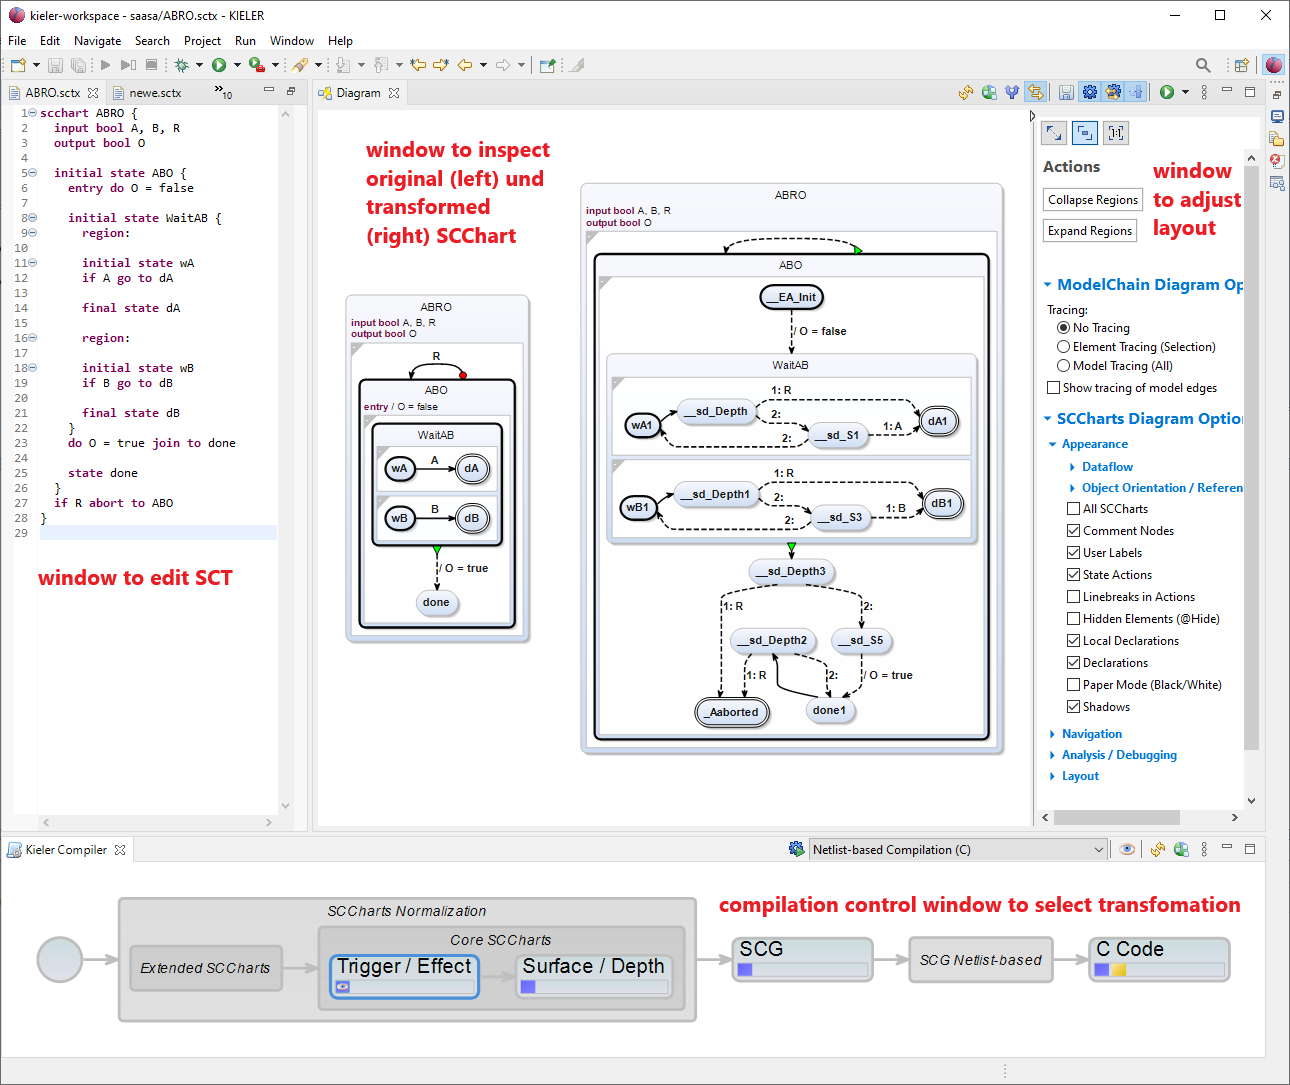
\includegraphics[width=1.0\textwidth]{bilder/KIELER_Tool_Screenshot.png}
\caption{Screenshot of KIELER SCCharts tool (adapted from~\cite{Motika.2017})}
\label{fig:KIELER_Tool_Screenshot}
\end{figure} 